\chapter{Problemløsning}\label{ch:chlabel}
I dette kapitel vil løsningen til problemformuleringen blive beskrevet og argumenteret for. Der bliver stillet krav til programmet for at løse problemet på den bedste måde. Ud fra disse krav vil der blive designet et program som løsning på problemformuleringen. Til sidst forklares det, hvordan dette design er implementeret, gennem programmeringen og datastrukturen. Der gives også beskrivelser og forklaringer af flere af de centrale funktioner fra kildekoden. 

% Ret eller omformuler endelig hvis du har noget bedre
% det hvordan et program kan blive til en løsning, på det problem der er opstillet i problemformuleringen. Først ved at formulerer et antal konkrete krav til løsningen. Efterfølgende designes der et program ud fra disse krav. Til sidst forklares det hvordan dette design er implementeret, ved at beskrive programmeringsstil og datastruktur. Der gives også beskrivelse og forklaringer af flere funktioner fra kildekoden.

\section{Krav til løsningen}\label{afsnit:krav}
For at lave en funktionel løsning til projektets problemformulering, er det nødvendigt at opstille en række krav. Disse krav skaber rammen for de opgaver, løsningen skal være i stand til at udføre.\\
Et af de grundlæggende krav til løsningen er, at den skal være i stand til at opstille en stævneplan. Denne stævneplan skal overholde reglerne for stævner i Kidzliga floorball, som er stillet af Floorball Danmark \cite{kidzRegler}. Derfor er det nødvendigt at tage disse regler i betragtning, når en stævneplan bliver udarbejdet.
\par
I dette afsnit er de relevante regler beskrevet i rækkefølge efter prioritet. Prioriteringen bestemmer hvilke regler, der er vigtigst at overholde, og hvilke der kan undlades i tilfælde af, at det ikke er muligt at implementere dem alle.
\begin{itemize}
    \item \textit{En kamp varer seks minutter,\ og der skal være en til to minutters pause mellem hver kamp.} I forbindelse med projektet er det besluttet at sætte et krav om to minutters pause mellem hver kamp, da det er mere specifikt.
    \item \textit{Alle hold, der deltager, skal have cirka seks kampe.} Reglerne er i dette tilfælde heller ikke specificeret yderligere. Derfor er kravet i projektet gjort mere specifikt, ved at hvert hold skal have seks kampe. Kun hvis dette ikke er muligt, må et eller flere hold spille én kamp mere eller mindre. 
    \item \textit{Alle kampe i en runde skal startes og afsluttes på samme tid.} Denne regel er med til at sikre, at stævneplanen ikke skrider så meget, at et hold pludselig skal spille to steder på samme tid, eller meget kort tid efter hinanden, hvilket strider imod den følgende regel.
    \item \textit{Alle hold skal have mindst én hvilekamp mellem hver kamp}, hvis det er muligt. Er det ikke muligt at indlægge en hvilekamp, tilstræbes det ifølge reglerne, at holdet, der spiller flere runder i træk, spiller på samme bane. I dette projekt er det fastsat som en regel, at kampen skal foregå på samme bane, i tilfælde af at en hvilekamp ikke er mulig. 
    \item \textit{Et hold må kun spille mod et andet hold, der er på det samme niveau.} Der er defineret fire forskellige niveauer i Kidzliga: N, A, B og C. Niveauerne er delt op, C er det højeste niveau, så kommer B, A og til sidst N, som står for nybegynder. 
    \item Det kan forekomme, at en stævneplan bliver hængt op i en hal, hvor stævnet bliver afviklet. Derfor stilles der et krav til løsningen, om at \textit{den udviklede stævneplan skal være opstillet på en præsentabel måde.} Det er herudfra bestemt, at opdeling i runder skal fremstå tydeligt, hvor hver runde er opdelt i kampe. Her skal banenummer, niveau og startstid for hver runde også stå.
\end{itemize} 

Det er nødvendigt at overholde disse specifikke regler, da problemet er afgrænset til Kidzliga. Ydereligere, opstilles krav til løsningen, som ikke er direkte stillet af Floorball Danmark. Disse regler fremsættes for at øge kvaliteten af stævneplanen. Et menneske vil naturligt følge dem, men reglerne skal defineres klart, for at et program også overholder dem.
\begin{itemize}
    \item \textit{Et hold må ikke spille mere end 2 kampe i træk.} Dette er en udvidelse af reglen, om at der skal være en hvilkekamp mellem hver kamp og gælder, når dette ikke kan lade sig gøre. 
    \item \textit{Hvert hold skal spille mod et andet hold igen, så få gange som muligt, og to hold må ikke spille mod hinanden to kampe i træk.} Dette er besluttet for at sikre, at hvert hold kommer til at spille med så mange forskellige andre hold som muligt.
\end{itemize}
Disse regler skal overholdes for at få en stævneplan af høj kvalitet, men er ikke nødvendige at overholde for at få en fungerende stævneplan.
\\\\
Problemformuleringen nødvendiggør også et krav, om at stævneplanen skal være fleksibel. Det skal derfor være muligt at foretage ændringer i stævneplanen, efter den er blevet udarbejdet. Programmet skal tillade brugeren at tilføje og fjerne hold fra stævneplanen. Dette vil gøre stævneplanen mere fleksibel, da brugeren får mulighed for at lave hurtige ændringer i en allerede eksisterende stævneplan.
\\\\
Ved at specificerer kravene, er floorball-reglerne blevet mere konkrete. Der er hermed fastlagt et udgangspunkt for programmets overordnede design, der vil kunne bygges videre på for at løse problemet.

\clearpage

\section{Design}\label{afsnit:design}
Ud fra kravene er det muligt at designe et program til at løse problemstillingen. Designet er den overordnede ide, om hvordan programmet skal fungere og hænge sammen. Samtidigt afklarer designet, hvordan problemet kan deles op i flere, mere overkommelige opgaver, for at gøre det nemmere at udvikle og forstå programmet. 
\\\\
Der er blevet lavet tre flowcharts til at beskrive programmets design. \textit{Det overordnede flowchart} viser strukturen af programmet (se figur \ref{fig:overordnet-flowchart}). \textit{Lav ny stævneplan} (se figur \ref{fig:lav-flowchart}) viser tanken bag, hvordan programmet laver en stævneplan. Til sidst er der \textit{rediger stævneplan} (se figur \ref{fig:rediger-flowchart}), som viser, hvordan programmet skal kunne tilføje og fjerne hold fra en eksisterende stævneplan. Det overordnede flowchart bliver gennemgået først.

\begin{figure}[H]
  \centering
  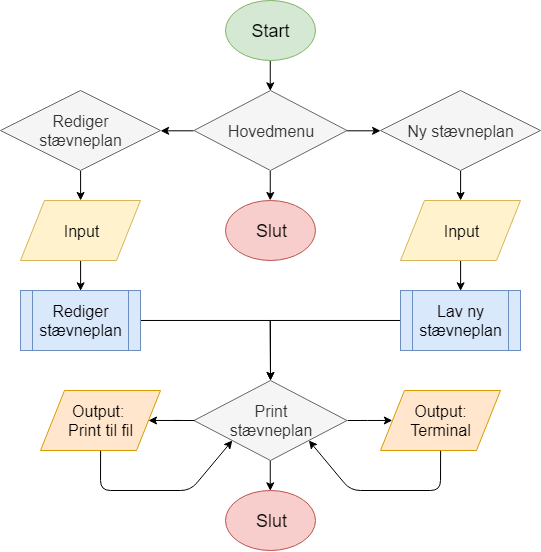
\includegraphics[width=0.7\textwidth]{figures/Overordnet_v2.png}
  \caption{Flowchart over programmets overordnede struktur. Der er tre grene, en for at lave en ny stævnplan, en for at redigere en eksisterende plan og en for at afslutte programmet.}
  \label{fig:overordnet-flowchart}
\end{figure}

På figur \ref{fig:overordnet-flowchart} ses den overordnede struktur over programmets opbygning. Programmet starter med en hovedmenu, hvor brugeren skal vælge mellem tre hovedgrene. Den højre gren (se figur \ref{fig:lav-flowchart}) giver mulighed for at lave en ny stævneplan, den venstre gren (se figur \ref{fig:rediger-flowchart}) giver mulighed for at redigere en allerede eksisterende stævneplan, og den sidste gren afslutter programmet. Disse valgmuligheder er med til at give et overblik over hvad programmet kan, og giver mulighed for at brugeren selv kan bestemme hvad de ønsker at gøre med programmet.

\subsubsection{Lav ny stævneplan}
Først gennemgås designet af hvordan en ny stævneplan oprettes. Løsningen skal være i stand til at overholde de opstillede krav for oprettelse af en stævneplan, og skal derfor bruge følgende informationer fra brugeren:
\begin{itemize}
    \item Holdnavne med niveau i en tekstfil
    \item Antal baner
    \item Starttidspunktet for stævnet
\end{itemize}
Disse informationer er nødvendige at have for at kunne lave en stævneplan, der er opstillet ordentligt og korrekt i overensstemmelse med de andre krav og regler. 
\par
Holdnavne og niveauer indlæses fra en tekstfil, da der kan være mange hold, og brugeren kan miste overblikket, hvis input tastes gennem terminalen. Når holdnavne skrives ind på en fil, bliver det mere overskueligt for brugeren. Dette kræver dog en specifik opsætning af filen, da programmet ellers ikke vil kunne læse den.
\\\\
% Beskrivelse af opsætningen
I eksemplet nedenfor fremstår det, at kravene til opsætningen er, at der skal være ét holdnavn på hver linje efterfulgt af et komma og holdets niveau. Holdnavnet må indeholde visse specialtegn (såsom "?!/\%-\_"\ mm.), men det første tegn skal være et bogstav. Niveauet, der angives med et bogstav, må være både stort og småt (se bilag \ref{ch:appIlabel}).
\\\\
Antallet af baner og starttidspunktet indlæses gennem terminalen, da disse er hurtigere for brugeren at taste ind.
\par
Nødvendige udregninger af inputet foretages, hvorefter brugeren skal tage et valg om der ønskes en stævneplan hurtigt eller om de ønsker en fejlfri plan. Dette er gjort muligt, da sammensætningen af en fejlfri stævneplan kan tage tid, som brugeren ikke nødvendigvis har på det tidspunkt, hvor programmet skal køres.
Herefter sammensættes stævneplanen. Dette sker ved brug af tilfældig sammensætning af kampe og runder, hvorefter hver runde evalueres, og der tælles fejl, i forhold til hvor mange gange de højest prioriterede regler er blevet brudt. Hvis runden ingen fejl har, godkendes den, ellers bliver den sammensat anderledes, indtil den er acceptabel. Hvis der ikke kan findes en rundesammensætning, som overholder de opstillede regler, startes processen igen fra første runde.
\par
Der var en overvejelse om at sammensætte stævneplanen på en struktureret måde, som en imitation af hvordan et menneske ville lægge planen, men gøre det hurtigere end en person kunne gøre det. Med denne metode er der dog en risiko, for at den bedste stævneplan ikke bliver fundet, da alle muligheder ikke nødvendigvis bliver udforsket. Ved at bruge den tilfældige metode, er der mulighed for at få sammensat flere forskellige stævneplaner tilfældigt, hvor den mest optimale udvælges.
\par
For at få det optimale resultat vil der være behov for et point-system, som giver point i forhold til de regler, der ikke er givet af Floorball Danmark. Jo flere regler der bliver opfyldt, jo flere point får stævneplanen. Hver stævneplan bliver hermed sammenlignet med den hidtil mest optimale, og den med flest point bliver gemt. Efter et fastsat antal iterationer bliver den bedste printet ud (se afsnit \ref{implementering}).
% \par
% Projektets program giver mulighed for at gøre dette, men det kan tage noget tid for programmet at komme frem til den bedste stævneplan. Dette skyldes, at for at stævneplanen bliver god nok, skal programmet køres et bestemt antal gange, som er meget stort, i forhold til den tid det tager for programmet at komme med en god stævneplan. Der er derfor også mulighed for at få lavet en stævneplan hurtigt, men hvor den ikke har lige så høj kvalitet som den anden mulighed.

% Det er dog ikke det projektets program gør, da denne løsning vil tage for lang tid for programmet at komme frem til den bedste stævneplan. Dette skyldes at for at stævneplanen bliver god nok, skal programmet køres et bestemt antal gange, som er for stort i forhold til den tid det tager for programmet at komme med en god stævneplan.

\begin{figure}[H]
  \centering
  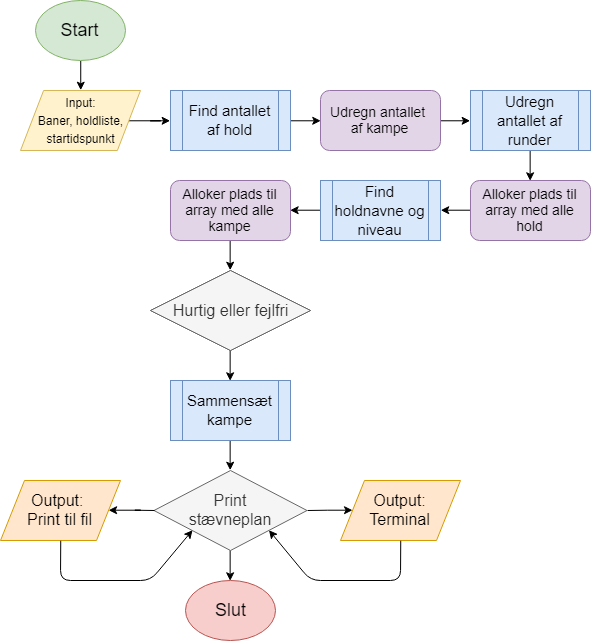
\includegraphics[width=0.7\textwidth]{figures/Lav_staevneplan.png}
  \caption{Flowchart over den første hovedgren af programmet. Her gives et overblik over processen for at lave en stævneplan.}
  \label{fig:lav-flowchart}
\end{figure}

Når en stævneplan skal sættes op, bliver brugeren bedt om at foretage et valg om hvilket output, der ønskes. Dette kan ses på figur \ref{fig:lav-flowchart}. Her er det muligt at få stævneplanen printet til terminalen, så brugeren har mulighed for at tjekke stævneplanens sammensætning, for at se om det er acceptabelt. Hvis brugeren ikke er tilfreds, kan der sammensættes en ny stævneplan fra hovedmenuen. Brugeren kan også få printet stævneplanen ud på en fil, da det er et krav, at man skal kunne printe stævneplanen ud og hænge den op i hallen.\\
Når brugeren er færdig med at lave stævneplanen, kommer de tilbage til hovedmenuen, ved at vælge afslut, hvor der igen er mulighed for at vælge mellem de tre grene på figur \ref{fig:overordnet-flowchart}.

\subsubsection{Rediger stævneplan}
Hvis brugeren vælger at redigere stævneplanen, følger man venstre hovedgren på figur \ref{fig:overordnet-flowchart}. Som det fremstår på det overordnede flowchart, gør løsningen det muligt for en bruger at redigere en allerede eksisterende stævneplan ved at tilføje eller fjerne hold. For at dette kan lade sig gøre, kræves det, at den eksisterende stævneplan er af samme format som programmet bruger.
% Indsæt rediger-kampprogram flowchart her!
\par
Måden hvorpå programmet redigerer en eksisterende stævneplan, er illustreret på figur \ref{fig:rediger-flowchart} (s. \pageref{fig:rediger-flowchart}). Først skal brugeren vælge hvilken ændring der ønskes at fortage. Vælges der at tilføje et hold, skal brugeren derefter indtaste antallet af hold der ønskes at tilføje, samt deres holdnavne og niveau. Disse informationer overføres til listen af hold for den eksisterende plan, der skal ændres. Efterfølgende kan der foretages flere ændringer, indtil brugeren er tilfreds. Der er også mulighed for at fjerne hold. Vælger man dette skal der indtastes antallet af hold, som skal fjernes, samt de tilhørende holdnavne. Disse hold bliver fjernet fra listen, som indeholder alle holdene fra den plan der skal redigeres.
\par
Herefter bearbejdes informationerne om holdene, så de stemmer overens med de ændringer, brugeren ønsker. Dette kan ses i kildekode \ref{code:updateTournament} side \pageref{code:updateTournament}. Til sidst fremstilles en stævneplan med ændringerne, på samme måde som der fremstilles en ny stævneplan. Brugeren har mulighed for at printe stævneplanen, enten i terminalen eller til en fil. I terminalen kan stævneplanen inspiceres, og der er mulighed for at lave yderligere ændringer eller generere en ny stævneplan, før den færdige plan gemmes.

\begin{figure}[H]
  \centering
  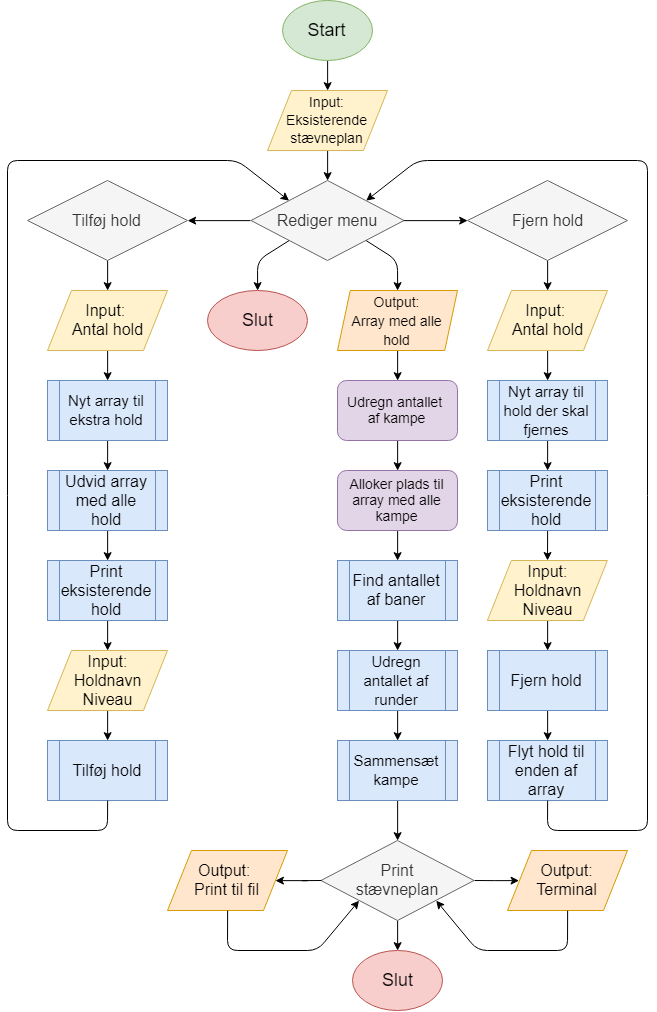
\includegraphics[width=0.7\textwidth]{figures/Rediger_staevneplan.png}
  \caption{Flowchart over den anden hovedgren af programmet. Her gives et overblik over processen for at redigere en allerede eksisterende stævneplan.}
  \label{fig:rediger-flowchart}
\end{figure}
% % % % % % % % % % % % % % % hest?

\clearpage

\section{Implementering}\label{implementering}
% Hvilke antagelser der er i forhold til at programmet skal kører ordentligt.
% Hvordan gør vi rent faktisk det her, helt nede i koden
% Forklaring af snippets
Dette afsnit handler om implementeringen af løsningen. Den måde koden er skrevet, tager udgangspunkt i det design, der er beskrevet i forrige afsnit. Den anvendte programmeringsstil beskrives ligeledes for nemmere at kunne læse kildekoden. Datastruktureren, der er brugt i kildekoden, forklares, og der argumenteres for trufne valg i denne forbindelse. Til sidst beskrives de mest centrale funktioner fra kildekoden, med tilhørende forklaringer og kodeeksempler. Dette gøres for at hjælpe læseren med at følge de tanker og ideer, der har været bag de valg, som er blevet truffet.

\subsection{Programmeringsstil}
Som programmeringsstil refereres der til en modificeret version af C Coding Standard \cite{codingstyle}. En af de modifikationer der er foretaget, er at betingelser, i eksempelvis if-else-kæder, har konstanten placeret til højre i stedet for til venstre, som standarden anbefaler. Et eksempel på dette kan ses i kodeeksempel \ref{code:conditionStyle} herunder.

\begin{listing}[H]
\begin{minted}[frame=lines, framesep=3mm, baselinestretch=1, linenos, bgcolor=LightGray]{c}
/* Som standarden foreskriver: */
if (0 == var) {
    ...
}

/* Som det gøres i dette projekt: */
if (var == 0) {
    ...
}
\end{minted}
\captionsetup{name=Kodeeksempel}
\captionof{Kodeeksempel}{Kodeeksempel, der viser forskellen i opsætningen af kontrolstrukturer mellem C Coding Standard \cite{codingstyle} (fra l. 2) og dette projekt (fra l. 7).}
\label{code:conditionStyle}
\end{listing}

\clearpage
Derudover skrives kommentarer ikke i slutningen af eksempelvis en if-else-kæde, som det er beskrevet i C Coding Standard. I stedet skrives disse i begyndelsen eller ved siden af (se kodeeksempel \ref{code:commentStyle}). Dette gøres så forklaringen kommer før koden for at øge læsbarheden.

\begin{listing}[H]
\begin{minted}[frame=lines, framesep=3mm, baselinestretch=1, linenos, bgcolor=LightGray]{c}
if (var == 0) {
    ...
} /* Som standarden foreskriver: */


/* Som det gøres i dette projekt: */
if (var == 0) {
    ...
    ...     /* Dette gøres også */
}
\end{minted}
\captionof{Kodeeksempel}{Kodeeksempel, der viser forskellen i placering af kommentarer mellem C Coding Standard \cite{codingstyle} (se linje 3), og dette projekt (se linje 6 og 9).}
\label{code:commentStyle}
\end{listing}

Det tilstræbes, at antallet af tegn per linje er 78 \cite{codingstyle}, da koden skal kunne passe på en A4-side. Der accepteres dog visse brud på denne regel i kildekoden. Dette skyldes, at nogle af programmets funktioner har mange parametre, og dermed overskrider de 78 tegn. 
\par
I kildekoden, er input, output og kommentarer skrevet på dansk, mens alt andet er skrevet på engelsk.
\par
Dette er ikke alle afvigelser, men det er de vigtigste for forståelsen af programmet. De andre medtages ikke, da de anses for meget små afvigelser.

\clearpage

\subsection{Datastruktur}
Udover en fast programmeringsstil i programmet, er der også opsat en fast datastruktur. Dette gøres, da det så bliver muligt at arbejde med problemet på en mere intuitiv og overskuelig måde. I dette afsnit, vil denne datastruktur blive beskrevet.
\par
Strukturen af Kidzliga stævner abstraheres i kildekoden til en samling af \textbf{\textit{match}}-structs, der hver repræsenterer en kamp. Hver af disse indeholder ligeledes en \textbf{\textit{team}}-struct for hvert hold i kampen. Stævnet er sat op som et array af \textbf{\textit{match}}-structs, der hver tildeles en bane og kan deles ind i runder. Niveauet bliver repræsenteret som et bogstav, men bliver reelt set behandlet som heltal, og derfor er det lavet til en enumeration type \textbf{\textit{levels}}.\\
Disse bliver gennemgået i de næste tre afsnit.

%Strukturen af Kidzliga stævner abstraheres i kildekoden til en samling af flere kampe, der er grupperet i runder. Der afvikles én kamp per bane i hver runde, og en kamp er en \textbf{\textit{match}}-struct, der består af to hold som er \textbf{\textit{team}}-structs, af samme niveau. 

\subsubsection{Hold struct}
En instans af \textbf{\textit{team}}-structen (se kildekode \ref{code:teamStruct}) indeholder al den information, der er relevant i forbindelse med et enkelt hold i et stævne. \\
Informationen er fordelt på structens members, der består af en streng med holdets navn, et heltal med antallet af kampe de har spillet og et heltal med holdets niveau.\\
Heltallet \textbf{\textit{games}} bruges til at holde styr på, at et hold spiller det rette antal kampe. Dette tal skal tælles op hver gang de bliver sat i en ny \textbf{\textit{match}}.

\begin{listing}[H]
\begin{minted}[frame=lines, framesep=3mm, baselinestretch=1, linenos, bgcolor=LightGray]{c}

typedef struct {
  char team[MAX_NAME_LEN];
  int games;
  int level;
} team;

\end{minted}
\captionof{listing}{Structen \textbf{\textit{team}}, som den er defineret i kildekoden. Denne struct representerer et hold og indeholder holdnavn (\textbf{\textit{team}}), antal kampe spillet (\textbf{\textit{games}}) og holdets niveau (\textbf{\textit{level}}).}
\label{code:teamStruct}
\end{listing}

\clearpage

\subsubsection{Kamp struct}
Structen \textbf{\textit{match}} (se kildekode \ref{code:matchStruct}) indeholder den information, der er relevant for en kamp. Informationen er, ligesom tidligere, fordelt på de enkelte members, der består af en \textbf{\textit{team}}-struct med det ene hold i kampen, en \textbf{\textit{team}}-struct med det andet hold i kampen, et heltal med niveauet for kampen og et heltal, der repræsenterer banen, hvorpå kampen afvikles. \\
De members, der indeholder de deltagende hold, er af den tidligere nævnte type \textbf{\textit{team}}. Dette gør det muligt at få adgang til information om holdene, der deltager i en given kamp, ved at tilgå disse instansers members.

\begin{listing} [H]
\begin{minted}[frame=lines, framesep=3mm, baselinestretch=1, linenos, bgcolor=LightGray]{c}

typedef struct{
  team team_a;
  team team_b;
  int level;
  int field;
} match;

\end{minted}
\captionof{listing}{Structen \textbf{\textit{match}}, som den er defineret i kildekoden. Denne struct representerer en kamp i stævneplanen og indeholder de to hold der spiller i kampen (\textbf{\textit{team\_a}} og \textbf{\textit{team\_b}}), kampens niveau (\textbf{\textit{level}}) og banen kampen spillet på (\textbf{\textit{field}}).}
\label{code:matchStruct}
\end{listing}

\subsubsection{Enumeration type}
Udover disse structs er der også defineret en enumeration type ved navn \textbf{\textit{levels}} (se kildekode \ref{code:levelEnum}). Grunden til dette er, at niveauerne, som de defineres i de officielle regler, er bogstaver. For at gøre det lettere at arbejde med i kildekoden kan disse bogstaver igennem denne enumeration type, konverteres til heltal. Grunden til at niveauet er repræsenteret som bogstaver, er fordi det står i floorball-reglerne, og er en bedre visuel repræsentation i input og output. 
\par
Der er en værdi yderligere i enumeration typen ved navn \textbf{\textit{EMPTY}}. Dette er nødvendigt for redigeringsdelen, da holdene struktureres i et array, hvor det ikke er muligt at slette hold, uden at lave et nyt array. Dette er mindre effektivt, da der skal allokeres mere plads og hvert ikke-tomt element skal kopieres. Brugen af arrayet vil blive uddybet senere i afsnittet. Hvis et element i dette array er "tomt", bliver holdets niveau sat til denne værdi, så de kan udelades når stævneplanen sammensættes.

\begin{listing}[H]
\begin{minted}[frame=lines, framesep=3mm, baselinestretch=1, linenos, bgcolor=LightGray]{c}

enum levels {EMPTY, N, A, B, C};

\end{minted}
\captionof{listing}{Enumeration typen \textbf{\textit{levels}}, som den er defineret i kildekoden. Hvert hold og kamp har et niveau: N, A, B eller C. \textbf{\textit{EMPTY}} gives til hold der ikke skal medtages i genereringen af stævneplanen.}
\label{code:levelEnum}
\end{listing}

Datastrukturen, der gøres brug af i dette projekt, består ikke kun i definitionen af nye datatyper. Selve stævnet, der som sagt består af en samling af kampe, er i kildekoden opstillet som et array med elementer af typen \textbf{\textit{match}}. Dette har til formål at samle alle kampene, så de er lette at overskue og arbejde med. Dette array er struktureret i rækkefølge, efter hvornår hver kamp finder sted. Denne struktur gør det muligt at udregne, hvilke kampe der er i hver runde, da der i hver runde spilles én kamp på hver bane. Derfor er det muligt at regne antallet af runder ud, hvis man kender antallet af baner, og det samlede antal kampe (se side \pageref{afsnit:createNewTournament}). Det er på en lignende måde muligt at udregne hvilken runde, en specifik kamp afvikles i: \[Kampens \ placering - (Kampens \ placering \ \textbf{mod} (antallet \ af \ baner))\]
Af denne grund er det ikke nødvendigt at opstille data efter runder.
\par
Ligeledes er alle holdene der deltager i stævnet, samlet i et array, med elementer af typen \textbf{\textit{team}}. Dette gøres så de er nemme at tilgå, når holdene skal sættes sammen i kampe.
\par
Når der i kildekoden arbejdes med et af de arrays, som er beskrevet ovenfor, eksempelvis i en funktion, sendes antallet af aktuelle, altså ikke-tomme, elementer også med. Dette gør det nemmere at arbejde med disse arrays, da det ikke er muligt at finde frem til størrelsen, når et array bruges i en funktion.
% Dette skyldes at der sendes en pointer til arrayet som inputparamenter, og ikke selve arrayet. Man ville derfor kunne finde størrelsen på denne pointer, men ikke størrelsen på arrayet.
\\\\
Disse datastrukturer bliver brugt gennem hele koden og er måden, information bliver sendt rundt mellem de forskellige funktioner, som kan ses i selve de udvalgte eksempler af kildekoden.

\clearpage

\subsection{Kildekodeeksempler}
I dette afsnit bliver der gennemgået forskellige udsnit af kildekoden i programmet. Denne kildekode vil blive forklaret, og der vil blive argumenteret for de valg, der er blevet taget under programmeringen.
\par
Programmet er lavet ud fra visse antagelser, om forholdene i stævnet. En af dem er, at der mindst er 10 hold i hvert niveau. Denne antagelse er nødvendig for, at et hold ikke kommer til at spille mod de samme modstandere for ofte. Desuden vil programmet ikke fungere optimalt hvis der er under 10 hold, da der ikke vil være nok mulige sammensætninger, og hvert hold må spille maks seks kampe.
\par
Der er også placeret en restriktion på maksimalt 9 baner. Det bliver en udfordring for programmet at sammensætte en korrekt stævneplan, hvis der er for mange baner i forhold til antallet af hold. Det antages at det er meget sjældent at et Kidzliga-stævne har mere end 9 baner til rådighed.
\par
På baggrund af disse antagelser bliver de vigtigste funktioner i programmet beskrevet, begyndende med funktionen createNewTournament, da denne funktion skal køres først for at lave en stævneplan.

\begin{figure}[H]
  \centering
  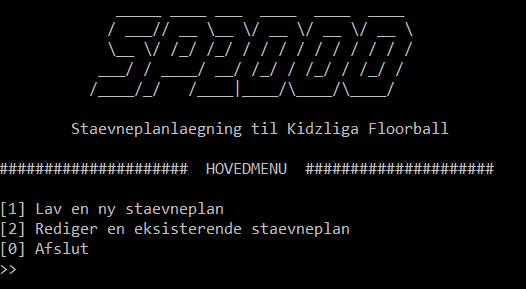
\includegraphics[width=0.7\textwidth]{figures/MainMenuScreenshot.PNG}
  \caption{Hovedmenu med programmets navn og de indledende valgmuligheder, lav ny stævne plan, rediger eksisterende stævneplan eller afslut program. Dette bliver præsenteret for brugeren når programmet bliver eksekveret.}
  \label{fig:mainmenu}
\end{figure}

\clearpage

\subsubsection{createNewTournament}\label{afsnit:createNewTournament}
I dette afsnit gennemgås \textbf{\textit{createNewTournament}}-funktionen med forklaringer og argumenter for den valgte implementering (se kildekode \ref{code:createNewTournament}). Når brugeren i hovedmenuen (se figur \ref{fig:mainmenu}) vælger at lave en ny stævneplan, indhenter programmet antallet af baner, starttidspunktet for stævnet og navnet på input-filen, som indeholder holdnavne og niveau, fra brugeren. 
Startstidspunktet omregnes fra timer og minutter, til minutter talt fra kl. 00:00. Dette udregnes af funktionen \textbf{\textit{promptForTime}} (se linje 16).
Input-filen skal indeholde en liste af holdnavne med tilhørende niveauer. Filen scannes to gange i løbet af funktionen. Først scannes den for at få antallet af hold, hvilket også svarer til antal linjer, der ikke er tomme, i filen (se linje 25).
\par
Variablen \textbf{\textit{number\_of\_matches}}, som angiver antallet af kampe, udregnes herefter. Dette gøres da det skal bruges til at udregne antallet af runder, der skal være i stævneplanen. Da kravene dikterer, at hvert hold skal spille 6 kampe, vil formlen se således ud:
\[\frac{6\ * \ number\_of\_teams}{2}\]
Der divideres med 2, da hver kamp indeholder to hold, og derfor tælles dobbelt i forhold til udregningen af antallet af kampe. (se linje 28)
\par
Funktionen \textbf{\textit{getNumberOfRounds}} (se linje 31) beregner antallet af runder ud fra \textbf{\textit{number\_of\_matches}}. Da der bruges heltalsdivision, risikeres der, at der overses en runde. Dette er dog ikke hensigtsmæssigt i forhold til udregningen, da der i nogle tilfælde vil mangle en runde. Funktionen undersøger derfor, om\[number\_of\_rounds \ \textbf{mod}(number\_of\_fields)\] er lig med nul. Hvis resten er lig med nul, kan der divideres uden ekstra tilføjelser. Formlen vil hermed se således ud:
\[\frac{number\_of\_matches}{number\_of\_fields}\]
Hvis resten ikke er lig nul, er der behov for at lægge 1 til resultatet for at få den manglende runde med, og formlen vil derfor være:
\[\frac{number\_of\_matches}{number\_of\_fields} + 1\]
\clearpage

\begin{source}
\begin{minted}[frame=lines, framesep=3mm, baselinestretch=1, linenos, bgcolor=LightGray]{c}
/* Sammensætter og printer en ny stævneplan fra bunden */
void createNewTournament(void) {
  FILE *fp = NULL;
  int number_of_fields = 0;
  int number_of_rounds = 0;
  int number_of_teams = 0;
  int number_of_matches = 0;
  int starting_time = 0;
  match *tournament = NULL;
  team *all_teams = NULL;
  char file_name[MAX_NAME_LEN];

  /* Prompter brugeren for antallet af 
     baner, startidspunkt og filnavn */
  number_of_fields = promptForFields();
  starting_time = promptForTime();
  promptForFileName(file_name);

  fp = fopen(file_name, "r");

  /* Check at filen blev fundet */
  isFileOpen(fp);

  /* Finder antallet af hold */
  number_of_teams = getNumberOfTeams(fp);

  /* Udregner antallet af kampe */
  number_of_matches = (number_of_teams * GAMES_PR_TEAM) / 2;

  /* Finder antallet af runder */
  number_of_rounds = getNumberOfRounds(number_of_matches, 
                                       number_of_fields);
                                       
  /* Allokerer plads til et array af alle hold */
  all_teams = allocateMemoryTeams(number_of_teams);

  /* Finder holdnavne og niveau i den åbne fil,
     og lægger dem over i all_teams */
  scanTeamFile(fp, file_name, number_of_teams, all_teams);


  /* Allokerer plads til et array 
     med plads til alle kampe der skal spilles */
  tournament = allocateMemoryMatch(number_of_matches);

  /* Sammensætter og evaluerer stævneplaner, 
     indtil der findes en der er acceptabel */
  generateTournament(number_of_teams, number_of_matches, 
                     number_of_fields, number_of_rounds, 
                     tournament, all_teams);

  /* Printer den færdige stævneplan, 
     enten til en fil eller til terminalen */
  printingMenu(tournament, starting_time, 
               number_of_rounds, number_of_fields);

  /* Frigør den hukommelse der er 
     allokeret til de forskellige arrays */
  free(all_teams);
  free(tournament);

  fclose(fp);

  return;
}
\end{minted}
\captionof{listing}{Funktionen \textbf{\textit{createNewTournament}}, der genererer og printer en ny stævneplan. \textbf{\textit{MAX\_NAME\_LEN}} er sat til 30. \textbf{\textit{GAMES\_PR\_TEAM}} er sat til 6.}
\label{code:createNewTournament}
\end{source}
\hspace{3 cm}
\begin{source}
\begin{minted}[frame=lines, framesep=3mm, baselinestretch=1, linenos, bgcolor=LightGray]{c}
/* Sammensætter og evaluerer stævneplaner, indtil der 
   findes en der er acceptabel. Der bruges enten en hurtig metode, 
   som bare kigger på om floorball regler bliver brudt
   eller den bedre metode som yderligere giver point 
   alt efter hvor god stævneplanen er */
void generateTournament(const int number_of_teams, 
                        const int number_of_matches, const int 
                        number_of_fields, 
                        const int number_of_rounds, 
                        match *tournament, team *all_teams) {
  int points = 0;
  int max_points = 0;
  int make_fast = 0;
  int no_go_count = 0;

  /* Udregner det maksimale antal point en stævneplan kan få,
     med de forudsætninger brugeren har stillet.
     Sætter derudover en fejlmargen på 5% */
  max_points = number_of_matches * 6 * 0.95;

  /* Prompter brugeren for at vælge mellem den hurtige metode, 
     eller finde den bedste stævneplan */
  make_fast = createMenu();

  /* Baseret på brugerens svar fra ovenstående funktion, 
     vælges metoden til generering af stævneplanen */
  if (make_fast == FAST) {
    do {
      no_go_count = createTournament(number_of_teams, 
                                     number_of_matches, 
                                     number_of_fields, 
                                     number_of_rounds, all_teams, 
                                     tournament, &points);
    } while (no_go_count != 0);
  }

  else if (make_fast == BEST) {
    while (!(no_go_count == 0 && points > max_points)) {

      points = 0;

      no_go_count = createTournament(number_of_teams, 
                                     number_of_matches, 
                                     number_of_fields, 
                                     number_of_rounds, all_teams, 
                                     tournament, &points);
    }
  }
}

\end{minted}
\captionof{listing}{Funktionen \textbf{\textit{generateTournament}}, der genererer en ny stævneplan.}
\label{code:generateTournament}
\end{source}
\clearpage
Herefter anvendes dynamisk pladsallokering til at lave et array \textbf{\textit{all\_teams}}, som vil indeholde en \textbf{\textit{team}}-struct for hvert hold (se linje 35). Dette gøres gennem funktionen \textbf{\textit{allocateMemoryTeams}}, hvor der bruges \textbf{\textit{malloc}}, da der ikke er behov for at nulstille elementerne i arrayet, før det bruges. Dette skyldes, at arrayets elementer alligevel bliver erstattet med \textbf{\textit{team}}-structs, så det er lige meget, hvad der tidligere var i det bestemte element. Overførslen af hold til \textbf{\textbf{all\_teams}} sker gennem \textbf{\textit{scanTeamFile}}-funktionen, som scanner filen med holdnavnene for at kopier dem over i arrayet.
\par
Der bliver brugt dynamisk allokering fremfor statisk allokering, fordi størrelsen på arrayet afhænger af \textbf{\textit{number\_of\_matches}}, som varierer i forhold til antallet af hold. Variablen \textbf{\textit{number\_of\_matches}} beregnes ud fra \textbf{\textit{number\_of\_teams}}, som afhænger af antallet af holdnavne, der står i filen. 
\par
Der bliver også allokeret plads til et \textbf{\textit{tournament}}-array (se linje 44). I dette array sættes de forskellige kampe ind, i den rækkefølge de vil fremstå i den endelige fil for stævneplannen. Der er to måder, hvorpå arrayet kan fyldes op. Dette bestemmes af brugeren, da den ene måde er hurtigere, men den anden skaber et resultat der opfylder kravene bedre (se afsnit \ref{afsnit:krav}). 
\\\\
Dette gøres gennem funktionen \textbf{\textit{generateTournament}} (se kildekode \ref{code:generateTournament}). Den hurtige metode fylder arrayet gennem en do-while løkke (se linje 27 i kildekode \ref{code:generateTournament}), som kalder funktionen \textbf{\textit{createTournament}}, der har til formål at sætte en stævneplan sammen, så de fastsatte krav, bliver overholdt. Er dette ikke muligt, returneres heltallet \textbf{\textit{no\_go\_count}}, som bestemmer, hvorvidt løkken skal køres igen.
\par
Variablen \textbf{\textit{no\_go\_count}} repræsenterer antallet af gange, et af de stillede krav ikke overholdes. Programmet er struktureret på en sådan måde, at så længe \textbf{\textit{no\_go\_count}} ikke er nul, kaldes \textbf{\textit{createTournament}} igen.
\\\\
Hvis det vælges at sammensætte arrayet, så den bedste stævneplan bliver fundet, sker dette gennem en while-løkke (se linje 37). Funktionen \textbf{\textit{createTournament}} kaldes også i denne del, men betingelserne for hvor lang tid løkken skal køre, er forskellige. Der bliver kigget på hvor mange point, der bliver givet til stævneplannen i forbindelse med de ekstra krav, der er blevet stillet til programmet (se afsnit \ref{afsnit:krav}). Løkken vil køre, så længe \textbf{\textit{no\_go\_count}} er forskellig fra nul, og pointene ikke er nået \textbf{\textit{max\_points}}. Denne variabel bestemmes ud fra følgende udregning:
\[(number\_of\_matches * 6) * 0,95\]
Dette tal er baseret på det maksimale antal point en stævneplan kan opnå, hvilket er tre point for hvert hold i hver kamp. Der er tilladt en fejlmargen på fem procent, da sandsynligheden for at der genereres en stævneplan, som er perfekt, inden for den afsatte tidsramme, er meget lille.
\par
Måden hvorpå point bliver givet, er ud fra de regler, som ikke er stillet af floorball. Når en runde evalueres, gives der point til hver kamp. Der gives fem point, hvis den forrige runde ikke indeholder begge hold fra den nuværende runde. Derudover gives der et ekstra point, hvis en et hold ikke spiller i forrige runde.
\par
Når \textbf{\textit{generateTournament}} returnerer \textbf{\textit{tournament}}-arrayet, skal stævneplanen printes ud til brugeren enten på en fil eller gennem terminalen som standard output. Dette gøres gennem funktionen \textbf{\textit{printingMenu}} (se linje 54).
\par
Det sidste, der sker i funktionen, er at den hukommelse, som er allokeret til de to arrays \textbf{\textit{all\_teams}} og \textbf{\textit{tournament}}, bliver frigivet, og filen med holdnavnene og niveauerne lukkes.

\subsubsection{createTournament}
Funktionen \textbf{\textit{createTournament}} (se kildekode \ref{code:createTournament}) bliver kaldt af \textbf{\textit{generateTournament}}. Formålet med \textbf{\textit{createTournament}} er at sætte kampe sammen til runder, der tilsammen danner stævneplanen.
\par
Efter de relevante variable er erklæret, allokeres der plads til to arrays, \textbf{\textit{team\_a}} og \textbf{\textit{team\_b}} (se linje 23, kildekode \ref{code:createTournament}). Disse bruges til at holde styr på hvilke hold, der spiller i hver kamp, i en given runde. Det ene array indeholder indekser for det første hold i hver kamp, og det andet indeholder indekser for det andet hold. Hvert element i de to arrays repræsenterer således en kamp, da elemententerne svarer til indekset i \textbf{\textit{all\_teams}}-arrayet for de hold, der spiller i hver kamp. Herved dannes der to lister med holdene i hver kamp, som nemt kan redigeres.
\\
Hver gang \textbf{\textit{createTournament}} kaldes, er det nødvendigt at nulstille \textbf{\textit{games}} fra \textbf{\textit{all\_teams}}-arrayet, da der startes forfra med sammensætningen af kampe i runder, og derfor er der ingen hold, der har spillet endnu. Dette gøres med funktionen \textbf{\textit{resetGamesPlated}} (se linje 28).
\par
I en for-løkke (se linje 33) dannes én runde af gangen. Indekset for den første kamp i den seneste runde, samt den nye runde, udregnes som produktet af rundenummeret og antal baner (se linje 35, kildekode \ref{code:createTournament}):
\[round\_count * number\_of\_fields\]

\clearpage

\begin{source}
\begin{minted}[frame=lines, framesep=3mm,baselinestretch=1, linenos, bgcolor=LightGray]{c} 
/* Sammensætter en stævneplan, og returnerer 
   antallet af gange planen bryder med floorball reglerne. */
int createTournament(const int number_of_teams, 
                     const int number_of_matches, 
                     const int number_of_fields, 
                     const int number_of_rounds, 
                     team *all_teams, match *tournament, 
                     int *points) {
                     
  int field_index = 0;
  int round_count = 0;
  int end_of_round = 0;
  int start_of_round = 0;
  int start_of_next_round = 0;
  int sentinel_count = 0;
  int no_go_count = 0;
  int temp_points = 0;
  int *team_a;
  int *team_b;

  /* Allokerer plads til to arrays, der indeholder indekser
     for det første og det andet hold i alle kampe */
  team_a = malloc (number_of_fields * sizeof(int));
  team_b = malloc (number_of_fields * sizeof(int));

  /* Nulstiller antallet af kampe hvert hold har spillet,
     hvis det allerede er forsøgt at generere en stævneplan */
  resetGamesPlayed(number_of_teams, all_teams);

  /* Sammensætter alle runder, en af gangen,
     og tjekker om de har brudt med regler, 
     og hvor mange point de får */
  for (round_count = 0; round_count < number_of_rounds; 
       round_count++) {
    start_of_round = round_count * number_of_fields;
    start_of_next_round = (round_count + 1) * number_of_fields;

    /* Sammensætter en enkelt runder, 
       og returnerer indekset for den sidste kamp i runden */
    end_of_round = createRound(start_of_next_round, start_of_round, 
                               number_of_teams, number_of_fields, 
                               team_a, team_b, all_teams, 
                               tournament);

    /* Tjekker om runder overholder reglerne. */
    no_go_count = evaluateRound(tournament, end_of_round, 
                                number_of_fields, &temp_points);

    /* Hvis runden ikke overholder reglerne sammensættes den på ny,
       indtil det er blevet forsøgt mere end CHECK_NUM gange */
    if (no_go_count > 0 && 
        sentinel_count < CHECK_NUM) {
      /* Sætter antallet af kampe tilbage til det 
         den var før runden blev sammensat. */
      for (field_index = 0; field_index < number_of_fields; 
           field_index++) {
        all_teams[team_a[field_index]].games--;
        all_teams[team_b[field_index]].games--;
      }

      /* Går én runde tilbage, og tæller flaget,
         der holder øje med antallet af forsøg, op med én */
      round_count--;
      sentinel_count++;

      /* Pointene runden fik, sættes tilbage til nul */
      temp_points = 0;
    }
    /* Hvis det er forsøgt tilstrækkeligt mange gange, 
       at sætte runden sammen, returneres 1, 
       så der prøves igen fra starten */
    else if (sentinel_count >= CHECK_NUM) {
      return 1;
    }
    /* Eller må det betyde at runden er gået igennem,
       og antallet af point den nuværende 
       stævneplan har fået, tælles op */
    else {
      *points += temp_points;
      temp_points = 0;
      sentinel_count = 0;
    }
  }

  free(team_a);
  free(team_b);

  /* Til sidst returners antallet af gange, 
     en floorball regel blev brudt */
  return no_go_count;
}
\end{minted}
\captionof{listing}{Funktionen \textbf{\textit{createTournament}}, der genererer en stævneplan og tjekker om den overholder de stillede krav. \textbf{\textit{CHECH\_NUM}} er sat til 100.000.}
\label{code:createTournament}
\end{source}

\hspace{3 cm}
\clearpage
\begin{source}
\begin{minted}[frame=lines, framesep=3mm, baselinestretch=1, linenos, bgcolor=LightGray]{c}
/* Sammensætter en runde  */
int createRound(const int start_of_next_round, 
                const int start_of_round, const int number_of_teams, 
                const int number_of_fields, int *team_a, int *team_b, 
                team *all_teams, match *tournament) {
                
  int tournament_index = 0;
  int match_index = 0;

  /* Gennemgår de kampe der skal være i runden, 
     og finder to hold der passer ind */
  for (tournament_index = start_of_round; tournament_index < 
       start_of_next_round; tournament_index++) {
    team_a[match_index] = findFirstTeam(tournament_index, 
                                        number_of_fields, 
                                        number_of_teams, all_teams, 
                                        tournament);
    team_b[match_index] = findSecondTeam(tournament_index, 
                                         number_of_teams, 
                                         all_teams, tournament);

    match_index++;
  }

  /* Returnerer det indeks runden stoppede ved */
  return tournament_index;
}
\end{minted}
\captionof{listing}{Funktionen \textbf{\textit{createRound}}, der sammensætter hold i kampe, så de stillede krav opfyldes. Dette gøres et antal gange svarende til antallet af baner, således at der dannes en runde af stævneplanen.}
\label{code:createRound}
\end{source}
\clearpage
Indekset for den sidste kamp i runden bliver returneret fra funktionen \textbf{\textit{createRound}} (se kildekode \ref{code:createRound}). Denne funktion går igennem hver kamp i runden og finder to tilfældige hold til at spille hver kamp. For at finde det første hold, kaldes funktionen \textbf{\textit{findFirstTeam}} (se kildekode \ref{code:findFirstTeam}), som producerer et tilfældigt tal ud fra tidspunktet programmet køres, og finder resten ved division med antal hold (se linje 14):
\[rand() \ \textbf{mod}(number\_of\_teams)\]
Således opnås et tal indenfor intervallet af indekser i \textbf{\textit{all\_teams}}-arrayet. Herefter tjekkes det, om holdet med dette indeks kan spille i kampen (se linje 18, kildekode \ref{code:findFirstTeam}). Hvis holdet endnu ikke har spillet seks kampe, og dets niveau ikke er sat til \textbf{\textit{EMPTY}}, kopieres holdnavn og niveau over i kampen i \textbf{\textit{match}}-structen for den gældende kamp (se linje 22). Desuden findes den bane kampe skal afvikles på, som også gemmes i kampen (se linje 24).
\par
For hvert tilfældigt genereret tal, der ikke opfylder kravene i if-sætningen, tælles flaget \textbf{\textit{sentinel}} op med én. Flaget bruges som kontrolvariabel. Hvis et tal, der overholder if-sætningens regler bliver fundet, sættes flaget til et tilstrækkeligt stort tal, da while-løkken (se linje 12) fortsætter så længe flaget er under dette tal. Dette gøres for at sikre at while-løkken ikke kører uendeligt. Den stoppes enten fordi et passende hold er fundet, eller den har været igennem løkken så mange gange at det antages, at der ikke findes et hold, der overholder reglerne. 
\clearpage
\begin{source}
\begin{minted}[frame=lines, framesep=3mm, baselinestretch=1, linenos, bgcolor=LightGray]{c}
/* Finder det første hold til en kamp. */
int findFirstTeam(const int tournament_index, 
                  const int number_of_fields, 
                  const int number_of_teams, 
                  team *all_teams, match *tournament) {
                  
  int sentinel_count = 0;
  int team_index = 0;

  /* Bliver ved med at lede efter et hold, indtil det er sikkert
     at der ikke kan findes et hold der passer med kriterierne */
  while (sentinel_count < CHECK_NUM) {
    /* Finder indekset til et tilfældigt hold i all_teams */
    team_index = rand() % number_of_teams;

    /* Tjekker om holdet der er fundet, har spillet under 6 kampe
       og dets niveau ikke er EMPTY, altså fjernet */
    if (all_teams[team_index].games < GAMES_PR_TEAM && 
        all_teams[team_index].level > EMPTY) {
      /* Hvis dette er sandt, kopieres det over i kampen, 
         og dets indeks returneres */
      tournament[tournament_index].team_a = all_teams[team_index];
      tournament[tournament_index].level = all_teams[team_index].level;
      tournament[tournament_index].field = tournament_index % 
                                           number_of_fields;
      all_teams[team_index].games++;
      return team_index;
    }
    sentinel_count++;
  }

  /* Hvis det ikke var muligt at finde et hold der passede,
     returneres indekset for det hold der nu er */
  return team_index;
}
\end{minted}
\captionof{listing}{Funktionen \textbf{\textit{findFirstTeam}}, der finder det første hold i en given kamp og tjekker at den overholder de stillede krav. \textbf{\textit{CHECH\_NUM}} er sat til 100.000. \textbf{\textit{GAMES\_PR\_TEAM}} er sat til 6. \textbf{\textit{EMPTY}} er af enumerationtypen \textbf{\textit{levels}} og svarer til heltallet 0.}
\label{code:findFirstTeam}
\end{source}
\clearpage
Funktionen \textbf{\textit{findSecondTeam}} (Den interesserede læser henvises til kildekoden, "tournamentCreate.c") finder på lignende vis det andet hold i kampen, dog er kriterierne for et hold, der kan spille i kampen, lidt anderledes. If-sætningen, der skal finde det andet hold, er sand, når dette hold er forskellig fra, men har samme niveau som, det første hold, og det har spillet mindre end seks kampe.
\par
% Begge hold kopieres derefter over i \textbf{\textit{tournament}}-arrayet på den næste ledige plads (se linje X, kildekode \ref{code:createRound}). \\
Når to hold er fundet til alle kampene i runden, returnerer \textbf{\textit{createRound}} indekset i \textbf{\textit{tournament}}-arrayet for den sidste kamp i runden. Yderligere returneres \textbf{\textit{team\_a}}, \textbf{\textit{team\_b}} og \textbf{\textit{tournament}}-arrayene, igennem output-parametrene til funktionen.
\par
Efter runden er dannet, evalueres den i funktionen \textbf{\textit{evaluateRound}} (se linje 46)(Den interesserede læser henvises til kildekoden, "tournamentCreate.c", for yderligere uddybelse). Her erklæres \textbf{\textit{no\_go\_count}}, der skal tælle antallet af gange runden ikke overholder de fastsatte regler (se afsnit \ref{afsnit:krav}). Hver kamp i runden gennemgås, og to if-sætninger tæller \textbf{\textit{no\_go\_count}} op, hvis et af holdene i kampen allerede spiller i runden, hvis de spiller i runden før, men ikke på samme bane eller hvis de har spillet i mere end to runder i træk. Herefter returneres værdien af \textbf{\textit{no\_go\_count}}.
\par
Der bliver desuden givet point baseret på de ekstra krav, der bliver opfyldt (se afsnit \ref{afsnit:createNewTournament} side \pageref{afsnit:createNewTournament}).
\par
Hvis \textbf{\textit{no\_go\_count}} er større end nul (se linje 51), betyder det at mindst én af kampene i runden ikke lever op til kravene. Der trækkes derfor én fra \textbf{\textit{games}} for de hold der var i runden, så de alligevel ikke har spillet den. Variablen \textbf{\textit{round\_count}}, der tæller antallet af runder, som indtil videre er dannet, tælles også én ned, hvilket medfører at runden bliver genereret på ny. Her sikrer flaget \textbf{\textit{sentinel\_count}}, at rundedannelsen ikke løber uendeligt. \\
Når alle runder er dannet succesfuldt, frigøres de arrays, der inderholder indekser for hold a og hold b, og \textbf{\textit{no\_go\_count}} bliver returneret fra funktionen. 

\clearpage

\begin{figure}[H]
  \centering
  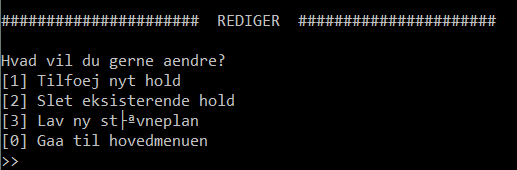
\includegraphics[width=0.7\textwidth]{figures/EditMenuScreenshot.PNG}
  \caption{Menuen der bliver præsenteret for brugeren når de vælger at redigere et kampprogram. Brugeren kan her vælge at tilføje hold, fjerne hold, generere en stævneplan ud fra de foretagede ændringer eller gå tilbage til hovedmenuen.}
  \label{fig:editmenu}
\end{figure}

\subsubsection{updateTournament}
I dette afsnit gennemgås \textbf{\textit{updateTournament}}-funktionen, med forklaringer og argumenter for den valgte implementering (se kildekode \ref{code:updateTournament}).
\par
Denne funktion kaldes i \textbf{\textit{mainMenu}} (Den interesserede læser henvises til kildekode, "menus.c"), hvis brugeren vælger at redigerer en eksisterende stævneplan. Funktionen kaldes med en enkelt parameter, der er en fil-pointer til en eksisterende stævneplan. Dette format er beskrevet i designafsnittet (se afsnit \ref{afsnit:design}).
\par
Efter initialiseringen af variablerne, findes antallet af hold, der allerede deltager i stævnet ved at kalde \textbf{\textit{getNumberOfTeamsTournament}} (se linje 14), som tæller antallet af unikke holdnavne i stævneplanen. 
\par
Herefter bliver brugeren præsenteret for en menu, printet af \textbf{\textit{editMenu}} (se figur \ref{fig:editmenu}), der giver muligheder for redigering af stævneplanen. Denne funktion returnerer et array \textbf{\textit{all\_teams}}, der indeholder alle de hold, der skal deltage i stævnet. Funktionen \textbf{\textit{modifyTeams}}, som er den funktion, der redigerer \textbf{\textit{all\_teams}}, og som bliver kaldt i \textbf{\textit{editMenu}}, bliver gennemgået på side \pageref{afsnit:modifyTeams}.
\par
Hvis brugeren ikke ønsker at lave ændringer, vil \textbf{\textit{all\_teams}}-array forblive NULL. Hvis dette er tilfældet, skal \textbf{\textit{updateTournament}} ikke foretage sig mere. Derfor tjekkes der i linje 21, om arrayet stadig er NULL. Hvis det er tilfældet, returnerer funktionen 1, hvilket betyder, at der ikke blev foretaget ændringer.
\par
Ellers fortsætter programmet ved at udregne antallet af kampe i stævnet (se linje 26). Her gøres brug af den samme formel som i afsnit \ref{afsnit:createNewTournament} på side \pageref{afsnit:createNewTournament}.
\par
Herefter starter processen med at lave en ny og opdateret stævneplan, ved at allokere plads til arrayet \textbf{\textit{tournament}}, som indeholder alle de kampe, der skal spilles i stævnet.
Denne pladsallokering udføres af \textbf{\textit{allocateMemoryTournament}} (se linje 29), som returnerer en pointer til det allokerede array.
\clearpage

\begin{source}
\begin{minted}[frame=lines, framesep=3mm, baselinestretch=1, linenos, bgcolor=LightGray]{c}
/* Opdaterer en eksisterende stævneplan, 
   ved enten at fjerne eller tilføje hold.
   Modtager en filpointer som er placeret i starten af filen. */
void updateTournament(FILE *fp) {
  int number_of_teams = 0;
  int number_of_matches = 0;
  int number_of_rounds = 0;
  int number_of_fields = 0;
  int starting_time = 0;
  team *all_teams = NULL;
  match *tournament = NULL;

  /* Finder antallet af hold i den eksisterende stævneplan. */
  number_of_teams = getNumberOfTeamsTournament(fp);

  /* Prompter brugeren for ændringer der skal laves */
  all_teams = editMenu(fp, all_teams, &number_of_teams);

  /* Tjekker om brugeren vil tilbage til hovedmenuen.
     Hvis all_teams er NULL, vil brugeren ikke fortsætte */
  if (all_teams == NULL) {
    return;
  }

  /* Udregner antallet af kampe. */
  number_of_matches = (number_of_teams * GAMES_PR_TEAM) / 2;

  /* Allokerer plads til array med alle kampe */
  tournament = allocateMemoryMatch(number_of_matches);
  /* Finder antallet af baner der er i den eksisterende stævneplan */
  number_of_fields = getNumberOfFields(fp);
  /* Udregner antallet af runder */
  number_of_rounds = getNumberOfRounds(number_of_matches, 
                                       number_of_fields);

  /* Sammensætter og evaluerer stævneplaner, indtil der findes 
     en der er acceptabel, baseret på brugerens valg af metode */
  generateTournament(number_of_teams, number_of_matches, 
                     number_of_fields, number_of_rounds, 
                     tournament, all_teams);

  /* Printer den færdige stævneplan, 
     enten til en fil eller til terminalen */
  starting_time = getStartingTime(fp);
  printingMenu(tournament, starting_time, 
               number_of_rounds, number_of_fields);

  /* Frigører dynamisk lagerallokering. */
  free(all_teams);
  free(tournament);

  /* Sætter filpointeren tilbage til starten af filen */
  rewind(fp);
  return;
}
\end{minted}
\captionof{listing}{Funktionen \textbf{\textit{updateTournament}} til redigering at en stævneplan. Der genererer en ny stævneplan ud fra ændringer defineret af brugeren og en eksisterende stævneplan. \textbf{\textit{GAMES\_PR\_TEAM}} er sat til 6.}
\label{code:updateTournament}
\end{source}
For at opstille en stævneplan, er det nødvendigt at finde \textbf{\textit{number\_of\_fields}} og \textbf{\textit{number\_of\_rounds}}. Variablen \textbf{\textit{number\_of\_fields}} findes ved brug af \textbf{\textit{getNumberOfFields}} (se linje 31). Det antages at denne variabel ikke har ændret sig fra den originale stævneplan. Variablen \textbf{\textit{number\_of\_rounds}} udregnes (se linje 33) på samme måde som i \textbf{\textit{createNewTournament}} (se afsnit \ref{afsnit:createNewTournament}, side \pageref{afsnit:createNewTournament}).

\par
Brugeren bliver derefter spurgt om hvilken metode til generering af stævneplanen der ønskes, på sammen måde som da der skulle laves en ny stævneplan. Der er igen mulighed for at vælge mellem \textit{den hurtige stævneplan} og \textit{den bedste stævneplan} (se linje 23, kildekode \ref{code:generateTournament}).
\par
Med disse værdier kan stævnet sammensættes på ny af \textbf{\textit{generateTournament}} (se linje 38), sådan at den er justeret til de ændringer, brugeren ønskede.
\par
For at sætte tidspunkter ind når stævneplanen printes, er det nødvendigt at kende stævnets starttidspunkt. Det antages, at dette heller ikke har ændret sig, og derfor kan det findes i den den gamle stævneplan med \textbf{\textit{getStartingTime}} (se linje 44).
\par
Det er nu muligt at opstille en ny stævneplan, der tager højde for ændringerne. Dette gøres ved at kalde \textbf{\textit{printingMenu}} (se linje 45)(se figur \ref{fig:printmenu}), som giver brugeren mulighed for at se og gemme den nye stævneplan.
\begin{figure}[H]
  \centering
  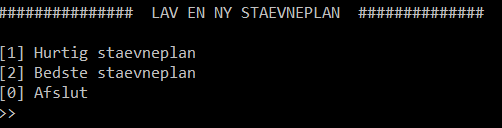
\includegraphics[width=0.7\textwidth]{figures/PrintingMenuScreenshot.PNG}
  \caption{Menuen der bliver præsenteret for brugeren når der skal printes en stævneplan}
  \label{fig:printmenu}
\end{figure}
\par
Til sidst frigøres den allokerede plads, og filpointeren sættes til at pege på starten af filen.

\subsubsection{Scan-funktioner}
Funktionerne \textbf{\textit{scanTeamFile}} (se kildekode \ref{code:scanTeamFile}) og \textbf{\textit{scanFileForTeams}} (se kildekode \ref{code:scanFileForTeams})\ scanner henholdsvis den oprindelige inputfil og en fil med en tidligere genereret stævneplan (se bilag \ref{ch:appIlabel} og \ref{ch:appHlabel}). Funktionen \textbf{\textit{scanTeamFile}} tager \textbf{\textit{all\_teams}}, hvor alle holdene placeres, som parameter. Dette array er tidligere i programmet blevet allokeret med \textbf{\textit{allocateMemoryTeams}}.
\par
Antallet af hold er tidligere fundet ved at tælle antallet af gange en linje i inputfilen succesfuldt kan scannes ind. Filen gennemgås igen, efter at filpointeren er ført tilbage til starten af inputfilen med funktionen \textbf{\textit{rewind}}. I denne gennemgang læses holdnavn og niveau over i deres respektive members af \textbf{\textit{team}}-structen for det gældende hold i \textbf{\textit{all\_teams}}-arrayet (se linje 18). Det sikres at \textbf{\textit{level}}, der er læst ind som en \textbf{\textit{char}}, er et stort bogstav, og derefter oversættes dette bogstav til et heltal, ved hjælp af enumeration-typen, som tidligere er defineret (se linje 22). Til sidst flyttes filpointeren tilbage til starten af inputfilen igen (se linje 29).
\\\\
Funktionen \textbf{\textit{scanFileForTeams}} (se kildekode \ref{code:scanFileForTeams}) starter med at flytte den relevante filpointer op til starten af inputfilen, med stævneplanen, og allokerer derefter plads til arrayet \textbf{\textit{all\_teams}} (se linje 12). Hver linje i filen læses over i et midlertidigt \textbf{\textit{char}}-array, som er statisk allokeret, så der er plads nok til hele linjen. En while-løkke fortsætter linje for linje, så længe det midlertidige \textbf{\textit{char}}-array der indlæses, ikke er \textbf{NULL} (se linje 14). En if-sætning tester, om hver linje er over \textbf{\textit{MIN\_LINE\_LEN}} tegn lang (se linje 18). Denne symbolske konstant er den mindste længde en linje kan have, hvis den indeholder informationerne for en kamp i stedet for en runde eller et tidspunkt. Her antages det, at linjer med runder og tid ikke indeholder whitespace, som gør linjen længere end 16 tegn lang. En stævneplan genereret af dette program vil overholde denne begrænsning, og det antages at brugeren ikke selv skriver inputfilen eller redigerer i den. Hvis dette ikke overholdes, kan der dog opstå problemer i kaldet af denne funktion. 

\clearpage

\begin{source}
\begin{minted}[frame=lines, framesep=3mm, baselinestretch=1, linenos, bgcolor=LightGray]{c}
/* Fylder et arrayet all_teams med holdnavne og niveau. */
void scanTeamFile(FILE *fp, const char *file_name, 
                  const int number_of_teams, team *all_teams) {
                  
  char level = ' ';
  int team_index = 0;

  /* Gennemgår filen med holdnavne, og kopierer holdnavn 
     og niveau over på de rigtige pladser i all_teams. */
  for (team_index = 0; team_index < number_of_teams; team_index++) {
    /* Checker om filpointeren er kommet til slutningen af filen,
       og stopper hvis det er sandt. */
    if (feof(fp)) {
      printf("EOF\nMulig fejl\n");
      break;
    }

    fscanf(fp, " %[a-zA-Z0-9 ] %*c %c", all_teams[team_index].team, 
                                        &level);

    /* Ændrer niveauet til stort bogstav. */
    level = toupper(level);
    /* Oversætter level fra char til int, 
       og gemmer denne i holdets level member */
    all_teams[team_index].level = getLevel(level);
  }

  /* Sætter filpointeren til starten af stævneplanen */
  rewind(fp);
}
\end{minted}
\captionof{listing}{Funktionen \textbf{\textit{scanTeamFile}} danner et array med alle hold og deres niveau. Disse informationer scannes ind via en fil med holdnavne og niveauer.}
\label{code:scanTeamFile}
\end{source}

\clearpage

\begin{source}
\begin{minted}[frame=lines, framesep=3mm, baselinestretch=1, linenos, bgcolor=LightGray]{c}
/* Scanner en stævneplan, returnerer et array med alle holdene. */
team *scanFileForTeams(FILE *fp, const int number_of_teams) {
  int scanres = 0;
  int team_index = 0;
  char temp[MAX_LINE_LEN];
  char temp_teams[MAX_LINE_LEN];
  char level;
  match temp_match;
  team *all_teams = NULL;

  /* Allokerer plads til et array med alle hold */
  all_teams = allocateMemoryTeams(number_of_teams);

  while (fgets(temp, MAX_LINE_LEN, fp) != NULL) {

    /* Hvis linjen er længere end MIN_LINE_LEN, 
       må den indeholde en kamp. */
    if (strlen(temp) > MIN_LINE_LEN) {
      scanres = sscanf(temp, 
                       " Bane %*d | %c | %[a-zA-Z0-9æøåÆØÅ ] ", 
                       &level, temp_teams);

      /* Hvis der ikke blev fundet et nivaeu og to hold i linjen */
      if (scanres != 2) {
        perror("Error scanning matches");
      }

      /* Konverterer niveauet fra char til int */
      temp_match.level = getLevel(level);

      /* Splitter holdene i strengen til to forskellige hold */
      splitTeams(temp_teams, &temp_match);

      /* Indsæt hold, hvis de ikke er i all_teams allerede. */
      copyNonExistingTeam(all_teams, temp_match.team_a, 
                          temp_match.level, &team_index);
      copyNonExistingTeam(all_teams, temp_match.team_b, 
                          temp_match.level, &team_index);
    }
  }

  /* Sætter filpointeren tilbage til starten af stævneplanen */
  rewind(fp);
  return all_teams;
}
\end{minted}
\captionof{listing}{Funktionen \textbf{\textit{scanFileForTeams}} danner et array med alle hold og tilhørende niveau. Disse informationer scannes ind fra en fil med en eksisterende stævneplan. \textbf{\textit{MAX\_LINE\_LEN}} svarer til 200. \textbf{\textit{MIN\_LINE\_LEN}} svarer til 16.}
\label{code:scanFileForTeams}
\end{source}

Funktionen \textbf{\textit{sscanf}} læser niveau og hvilke hold der spiller i kampen, over i henholdvis variablen \textbf{\textit{level}} og et midlertidigt \textbf{\textit{char}}-array (se linje 19). Banenummeret skal ikke bruges, så der anvendes assignment suppression (se linje 20), som scanner banenummeret uden at læse heltallet over i en variabel. Funktionen \textbf{\textit{sscanf}} returnerer antal gange der er blevet læst noget over i en variabel, og tæller derfor ikke \%*d med. Denne værdi føres over i \textbf{\textit{scanres}}, og det sikres at denne er lig med to (se linje 24), hvilket betyder en succesfuld indlæsning. Hvis dette ikke er tilfældet, printes en fejlmeddelelse. 
\\
Variablen \textbf{\textit{level}} oversættes til et heltal, ved hjælp af enumeration-typen for \textbf{\textit{levels}}, og overføres til \textbf{\textit{level}}-memberet af structen for den gældende kamp (se linje 29).
\par
Funktionen \textbf{\textit{splitTeams}} (se linje 32) går strengen, med de to hold der har spillet mod hinanden, igennem og leder efter et "\ vs "\ med mellemrum på begge sider. Dette bruges til at skille de to holdnavne ad og kopiere dem over i en midlertidig \textbf{\textit{match}}-struct, som returneres gennem output-parameterne til funktionen. Det antages at "\ vs "\ ikke bruges i navngivningen af hold (Den interessede læser henvises til kildekoden "printPrompt.c").
\par
Når den midlertidige \textbf{\textit{match}}-struct er dannet, tjekkes det, om de to hold allerede er i \textbf{\textit{all\_teams}}-arrayet (se linje 35), og ellers kopieres holdnavn og niveau for kampen over i den næste \textbf{\textit{team}}-struct i arrayet (Den interessede læser henvises til kildekoden "printPrompt.c"). 
\par
Til sidst sættes filpointeren igen tilbage til starten af input filen, så den er klar, hvis filen skal scannes igen. Funktionen returnerer det færdige \textbf{\textit{all\_teams}}-array.

\clearpage

\subsubsection{PrintProgram}
Funktionen \textbf{\textit{printProgram}} tager en filpointer som parameter. Når funktionen kaldes, er denne filpointer enten til outputfilen til stævneplanen, eller til \textbf{\textit{stdout}}. Når funktionen printer, bruges \textbf{\textit{fprintf}}, som typisk printer til en fil. Filpointeren \textbf{\textit{stdout}} peger på terminalen, og fungerer som en altid åben fil. 
\par
Funktionen \textbf{\textit{printProgram}} går gennem hver kamp i \textbf{\textit{tournament}}-arrayet, så længe begge hold i kampen starter med et bogstav (se linje 18). For hver kamp udregnes det nuværende tidspunkt, talt i minutter fra klokken 00:00, til timer og minutter i hver deres variabel (se linje 21).
\par
Hvis \textbf{\textit{number\_of\_fields}} går op i indekset for den gældende kamp (se linje 25), er denne kamp starten af en ny runde, da \textbf{\textit{number\_of\_fields}} svarer til hvor mange kampe, der spilles hver runde. Hvis det er starten på en ny runde, printes denne ud, efterfulgt af tiden for hvornår runden starter. Den første runde vil starte på det tidspunkt, brugeren tidligere har indtastet. Efterfølgende tælles tiden op med så mange minutter som en kamp og den efterfølgende pause tager, svarende til otte minutter (se linje 40). Variablen \textbf{\textit{round\_index}}, som er indekset for runden, tælles også op med én (se linje 41). 
\par
Det næste, der printes, er den næste kamp i \textbf{\textit{tournament}}-arrayet. Hvis \textbf{\textit{number\_of\_fields}} ikke går op i indekset for kampen (se linje 45), printes kampen kun, uden rundenummer og tid. Efter den sidste kamp i en runde, printes et ekstra linjeskift for at øge læsbarheden af stævneplanen. 
\par
Hver linje i den printede plan repræsenterer en kamp. Linjerne starter med hvilken bane kampen spilles på, efterfulgt af niveauet for holdene, og navnene på disse hold. For hver kamp der printes, tælles \textbf{\textit{match\_index}}, som er indekset for kampene, op med én. \\
% Meget pludselig afslutning, skal vi gøre noget ved dette? Jeg ved nemlig ikke hvor meget opsamlinger giver mening i de her afsnit... venlig hilsen Liv~=[,,_,,]:3

\clearpage

\begin{source}
\begin{minted}[frame=lines, framesep=3mm, baselinestretch=1, linenos, bgcolor=LightGray]{c}
/* Printer stævneplanen. Ud fra brugerens valg ved kaldstedet,
   printes stævneplanen enten til "staevneplan.txt" 
   eller til skærmen, stdout */
int printProgram(FILE *fp, const match *tournament, 
                 const int starting_time, 
                 const int number_of_rounds, 
                 const int number_of_fields) {
                 
  int round_index = 0;
  int match_index = 0;
  int hour = 0;
  int minute = 0;
  int time = starting_time;

  /* Chekker om et givent index i turnerings arrayet 
      indeholder gyldige hold. Afgjort ved at navnet 
      starter med et bogstav */
  while (isalpha(tournament[match_index].team_a.team[0]) != 0 && 
         isalpha(tournament[match_index].team_b.team[0]) != 0) {
    /* Udregner starttidspunktet for den nuværende runde */
    hour = time / 60;
    minute = time % 60;

    /* Hvis det er den første kamp i runden */
    if (match_index % number_of_fields == 0) {
      /* Printer runde nummer og tidspunktet 
         for hvornår der skal spilles */
      fprintf(fp, "Runde %d:\n%.2d:%.2d\n", round_index + 1, 
                                            hour, minute);
      /* Printer banenummer, niveau og holdene 
         der skal spille mod hinanden */
      fprintf(fp, "Bane %2d | %c | %s vs %s\n", 
              tournament[match_index].field + 1, 
              translateToChar(tournament[match_index].level),
              tournament[match_index].team_a.team, 
              tournament[match_index].team_b.team);

      /* Tidspunktet for den næste runde tælles 
         op med længden af én runde */
      time += ROUND_LEN;
      round_index++;
    }

    /* Hvis det er den sidste kamp i runden */
    else if (match_index % number_of_fields == number_of_fields - 1) {
      fprintf(fp, "Bane %2d | %c | %s vs %s\n", 
              tournament[match_index].field + 1, 
              translateToChar(tournament[match_index].level),
              tournament[match_index].team_a.team, 
              tournament[match_index].team_b.team);
      fprintf(fp, "\n");
    }

    /* Hvis det hverken er den sidste eller den første kamp i runden */
    else {
      fprintf(fp, "Bane %2d | %c | %s vs %s\n", 
              tournament[match_index].field + 1, 
              translateToChar(tournament[match_index].level),
              tournament[match_index].team_a.team, 
              tournament[match_index].team_b.team);
    }
    match_index++;
  }
  /* Sætter filpointeren til 
     starten af stævneplanen */
  rewind(fp);
  return 0;
}
\end{minted}
\captionof{listing}{Funtionen \textbf{\textit{printProgram}} printer den genererede stævneplan ud til enten terminalen eller en fil. \textbf{\textit{ROUND\_LEN}} svarer til otte minutter.}
\label{code:printProgram}
\end{source}

\clearpage

\subsubsection{modifyTeams}\label{afsnit:modifyTeams}
I dette afsnit vil funktionen \textbf{\textit{modifyTeams}} blive gennemgået og diskuteret. Funktionen kan ses i kildekode \ref{code:modifyTeams}.
\par
Funktionen \textbf{\textit{modifyTeams}} bliver kaldt i funktionen \textbf{\textit{editMenu}}. Her får brugeren muligheden for at tilføje eller fjerne hold. Alt efter hvad brugeren vælger, vil \textbf{\textit{modifyTeams}} blive kaldt med forskellige parametre der ændrer på den måde den behandler arrayet \textbf{\textit{all\_teams}}.
\par
Funktionen \textbf{\textit{modifyTeams}} kaldes enten med \textbf{\textit{ADD}} eller \textbf{\textit{REMOVE}}, som bestemmer, om der enten skal tilføjes eller fjernes hold. Disse to værdier er enumerationer, der står for henholdsvis 1 og 0. Tallene er arbitrære, da der bare skal være forskel på dem. Yderligere kaldes \textbf{\textit{modifyTeams}} enten med funktionen \textbf{\textit{copyTeams}} eller \textbf{\textit{deleteTeams}} som inputparameter, der bruges, når \textbf{\textit{all\_teams}} skal behandles.
\par
Det første, der sker, efter \textbf{\textit{modifyTeams}} bliver kaldt, er at brugeren bliver spurgt om antallet af hold, de vil tilføje eller fjerne. Dette bliver gjort med funktionen \textbf{\textit{promptForNumberOfTeams}}, som tager konstanten \textbf{\textit{modifier}} som inputparameter (se linje 13). Konstanten ændrer på, om brugeren vil blive spurgt, om hvor mange hold de vil tilføje, eller fjerne. 
\par
Efterfølgende bliver der allokeret hukommelse til \textbf{\textit{temp\_mod\_array}}, med plads til de hold, der skal ændres på (se linje 17). Derefter bliver der tjekket om brugeren valgte at tilføje hold, ved at se om \textbf{\textit{modifier}} er \textbf{\textit{ADD}} (se linje 21). Hvis dette er tilfældet, tælles variablen \textbf{\textit{number\_of\_teams}} op, og \textbf{\textit{all\_teams}} bliver re-allokeret til et større array ved brug af funktionen \textbf{\textit{updateTeams}} (se linje 23). Det er ikke nødvendigt at udvide \textbf{\textit{all\_teams}}, når der skal fjernes hold, da disse bliver markeret med \textbf{\textit{EMPTY}} og ignoreret af resten af programmet.
\par
Herefter bliver de nuværende hold printet til terminalen (se linje 27). Dette giver brugeren et overblik over, hvilke hold der allerede er i stævnet. Funktionen \textbf{\textit{printTeams}} printer holdene, og en af de inputparametre den får, er resultatet af en betinget operation (se linje 27 til 29). Hvis \textbf{\textit{modifyTeams}} skal tilføje hold, er \textbf{\textit{number\_of\_teams}} blevet talt op tidligere. Derfor er der brug for at trække \textbf{\textit{number\_of\_mod\_teams}} fra, da der ellers vil blive tilgået lagerplads udenfor \textbf{\textit{all\_teams}} (se linje 28). Hvis \textbf{\textit{modifyTeams}} derimod skal fjerne hold, har \textbf{\textit{number\_of\_teams}} ikke ændret sig, og funktionen kan blive kaldt uden at trække \textbf{\textit{number\_of\_mod\_teams}}.

\clearpage

\begin{source}
\begin{minted}[frame=lines, framesep=3mm, baselinestretch=1, linenos, bgcolor=LightGray]{c}
/* Ændrer på all_teams, baseret på funktionen *f 
   og konstanten modifier. Returnerer det ændrede all_teams */
team *modifyTeams(void (*f)(const team *, const int, const int, team *), 
                  const int modifier, team *all_teams, 
                  int *number_of_teams) {
                  
  team *temp_mod_array = NULL;
  int number_of_mod_teams = 0;

  /* Prompter brugeren for antallet af hold der skal fjernes 
     eller tilføjes. modifier bestemmer om der bliver printet 
     "tilføjes" eller "fjernes" til terminalen */
  number_of_mod_teams = promptForNumberOfTeams(modifier);

  /* Allokerer plads til et array med plads til de hold 
     der skal fjernes eller tilføjes */
  temp_mod_array = allocateMemoryTeams(number_of_mod_teams);

  /* Tjekker om all_teams skal udvides.
     Dette er kun nødvendigt når der tilføjes hold */
  if (modifier == ADD) {
    *number_of_teams += number_of_mod_teams;
    all_teams = updateTeams(all_teams, *number_of_teams);
  }

  /* Printer de nuværende hold til terminalen */
  printTeams(all_teams, (modifier == ADD) ? 
                        *number_of_teams - number_of_mod_teams : 
                        *number_of_teams);

  /* Prompter og scanner holdene, 
     der skal tiløjes eller fjernes, ind. */
  getTeams(number_of_mod_teams, *number_of_teams, all_teams, 
           modifier, temp_mod_array);

  /* Fjerner eller tilføjer hold, alt efter 
     hvilken funktion modifyTeams blev kaldt med */
  (*f)(temp_mod_array, number_of_mod_teams, 
       *number_of_teams, all_teams);

  /* Hvis der blev fjernet hold, 
     skal disse flyttes til bunden af all_teams */
  if (modifier == REMOVE) {
    sortArrayByLevel(all_teams, *number_of_teams);
    /* Antallet af hold tælles ned, så de hold 
       der blev fjernet, ikke kan tilgås */
    *number_of_teams -= number_of_mod_teams;
  }

  return all_teams;
}
\end{minted}
\captionof{listing}{Funktionen \textbf{\textit{modifyTeams}} laver ændringer i arrayet med hold der deltager i stævnet. Disse ændringer fortages på baggrund af brugerens valg, og kan bestå i enten at tilføje ller fjerne hold fra stævnet. \textbf{\textit{ADD}} og \textbf{\textit{REMOVE}} er af enumerationtypen \textbf{\textit{modifyer}} og indikerer henholdsvis at der tilføjes og fjernes hold. }
\label{code:modifyTeams}
\end{source}
\par
Efter brugeren har set hvilke hold, der er i den nuværende stævneplan, bliver funktionen \textbf{\textit{getTeams}} kaldt (se linje 33). Formålet med denne funktion er at få scannet de hold ind, der skal tilføjes eller fjernes. Hvis \textbf{\textit{modifyTeams}} er i gang med at tilføje hold, vil der yderligere blive scannet ind hvilket niveau hvert hold har (Den interessede læser henvises til kildekoden "tournamentUpdate.c"). Dette er ikke nødvendigt, når der skal fjernes hold, da funktionen \textbf{\textit{deleteTeams}} kun skal kende navnet på holdet. Navnene, og eventuelt niveauerne, på de hold, der skal tilføjes eller fjernes, bliver gemt i arrayet \textbf{\textit{temp\_mod\_array}}, som der blev allokeret plads til tidligere (se linje 17). 
\par
Når de hold, der skal tilføjes eller fjernes, er blevet fundet, kommer programmet til den funktion, som blev sendt ind som inputparameter (se linje 38). Her bliver \textbf{\textit{copyTeams}} eller \textbf{\textit{deleteTeams}} kaldt, som tidligere beskrevet i starten af dette afsnit. Funktionen \textbf{\textit{copyTeams}} kopierer holdene fra \textbf{\textit{temp\_team\_array}} over i de tomme pladser i \textbf{\textit{all\_teams}}. Funktionen, \textbf{\textit{deleteTeams}}, tager holdene fra \textbf{\textit{temp\_team\_array}} og sammenligner dem med holdene i \textbf{\textit{all\_teams}}, indtil den finder et match. Dette hold bliver så markeret med \textbf{\textit{EMPTY}}.
\par
Til sidst bliver der tjekket, om programmet skal fjerne hold (se linje 43). Hvis dette er tilfældet, sorteres holdene, således at de hold der er markeret med \textbf{\textit{EMPTY}}, kommer ned i bunden af \textbf{\textit{all\_teams}}. Variablen \textbf{\textit{number\_of\_teams}} bliver talt ned, så de hold ikke længere bliver talt med, når der senere skal sammensættes kampe. På denne måde er de praktisk taget blevet fjernet fra programmet, da de ikke længere bliver tilgået. 
\par
Herefter returneres \textbf{\textit{all\_teams}} til funktionen \textbf{\textit{editMenu}}, hvor brugeren så kan vælge at køre \textbf{\textit{modifyTeams}} igen. 


\subsection*{Opsamling} 
I dette afsnit er de vigtigste funktioner for programmet og løsningen af problemet blevet beskrevet og argumenteret for. 
\\\\
I de følgende kapitler vil projektet og programmet blive vurderet, konkluderet og perspektiveret. 
\par
I vurderingskapitlet (se kapitel \ref{ch:vurdering}), vil der blive vurderet om programmet opfylder de opstillede krav, samt afprøvet hvor hurtigt det genererer en stævneplan for hver af de to forskellige metoder til dette. Yderligere vil der også blive set nærmere på hvad der kunne gøres for at videreudvikle programmet så det bedre opfylde problemformuleringen.
\par
Konklusionskapitlet (se kapitel \ref{ch:konklusion}) konkluderer på de studiemæssige mål, og om problemformuleringen er opfyldt.
\par
I perspektiveringskapitlet (se kapitel \ref{ch:perspektivering}), bliver programmet sammenlignet med eksisterende værktøjer til sammensætning af stævneplaner. Yderligere udforskes alternative måder at løse problemet på, samt udvidelser af programmet, der eksempelvis kan øge dets målgruppe. 





% Skriv bl.a. om videreudvikling

%\subsection*{Noter}
%Vil vi generere noget tilfældigt, indtil vi finder det bedste, eller vil vi generere noget okay, og gøre det bedre?\\
%Genererer vi et helt kampprogram, og spørger om det er godt, eller genererer vi en enkelt runde, og spørger om den er god?